\documentclass{beamer}
\usepackage[utf8]{inputenc}
\usepackage[T1]{fontenc}
\usepackage{lmodern}
\usepackage{graphicx}
\usepackage{amsmath}
\usepackage{listings}
\usepackage{xcolor}
\usepackage{booktabs}
\usepackage{float}

% Code styling for listings
\lstdefinestyle{mystyle}{
	basicstyle=\ttfamily\footnotesize,
	backgroundcolor=\color{gray!10},
	frame=single,
	keywordstyle=\color{blue},
	commentstyle=\color{green!50!black},
	breaklines=true,
	numbers=left,
	numberstyle=\tiny\color{gray},
	captionpos=b
}
\lstset{style=mystyle}

\title{Fantasy Football Optimization}
\subtitle{Student Project: Global and Multi-Objective Optimization}
\author{Marco De Rito (SM3800016) \\ \small{Generated by a student, not by AI}}
\institute{University of Trieste}
\date{2025}

\begin{document}
	
	%%%%%%%%%%%%%%%%%%%%%%%%%%%%%%%%%%%%%%%%%%%%%%%
	\begin{frame}
		\titlepage
	\end{frame}
	
	%%%%%%%%%%%%%%%%%%%%%%%%%%%%%%%%%%%%%%%%%%%%%%%
	\begin{frame}{Overview}
		\begin{itemize}
			\item \textbf{Context}: Fantasy Football team selection via \emph{inverse optimization}.
			\item \textbf{Methodologies}: Metaheuristics (PSO, DE, ES).
			\item \textbf{Objective}: Balance budget, positions, and performance to achieve the best score.
		\end{itemize}
	\end{frame}
	
	%%%%%%%%%%%%%%%%%%%%%%%%%%%%%%%%%%%%%%%%%%%%%%%
	\begin{frame}{Introduction}
		\begin{itemize}
			\item Fantasy Football involves managing teams under budget and positional constraints.
			\item \emph{Inverse Optimization} adapts the scoring function based on historical data.
			\item A multi-manager auction is used for player assignments.
		\end{itemize}
	\end{frame}
	
	%%%%%%%%%%%%%%%%%%%%%%%%%%%%%%%%%%%%%%%%%%%%%%%
	\begin{frame}{Theoretical Background}
		\begin{block}{Inverse Optimization}
			Adjusting the cost/reward function so that observed solutions appear near-optimal.
		\end{block}
		\begin{block}{Metaheuristics}
			\begin{itemize}
				\item \textbf{PSO}: Inspired by swarm behavior.
				\item \textbf{DE}: Evolves solutions using vector differences.
				\item \textbf{ES}: Uses Gaussian mutations with selection strategies.
			\end{itemize}
		\end{block}
	\end{frame}
	
	%%%%%%%%%%%%%%%%%%%%%%%%%%%%%%%%%%%%%%%%%%%%%%%
	\begin{frame}[fragile]{Scoring Function and Fitness Logic}
		\textbf{Player Scoring Function:} Computes the score based on:
		\begin{itemize}
			\item Goals, assists, yellow/red cards, rating, and penalties.
		\end{itemize}
		\vspace{0.5em}
		\textbf{Fitness Function:} Evaluates a bid vector with penalties for:
		\begin{itemize}
			\item Exceeding budget, unbalanced positions, etc.
		\end{itemize}
		\vspace{0.5em}
		\textbf{Example Code:}
		\begin{lstlisting}[language=Python, caption=score_player in utils.py]
			def score_player(player):
			goals = getattr(player, 'goals_scored', 0)
			assists = getattr(player, 'assists', 0)
			yellow_cards = getattr(player, 'yellow_cards', 0)
			red_cards = getattr(player, 'red_cards', 0)
			rating = getattr(player, 'fantasy_rating', 6.0)
			penalties = getattr(player, 'penalties_scored', 0)
			
			score = (0.5 * goals +
			0.2 * assists -
			0.05 * yellow_cards -
			0.1 * red_cards +
			0.2 * rating +
			0.2 * penalties)
			
			return score
		\end{lstlisting}
	\end{frame}
	
	%%%%%%%%%%%%%%%%%%%%%%%%%%%%%%%%%%%%%%%%%%%%%%%
	\begin{frame}[fragile]{Manager Strategies}
		Each manager uses a metaheuristic to generate bids:
		\begin{itemize}
			\item \textbf{PSO}: Using the \texttt{pyswarm} library.
			\item \textbf{DE}: Using \texttt{scipy.optimize.differential\_evolution}.
			\item \textbf{ES}: Implemented via \texttt{deap}.
		\end{itemize}
		\vspace{0.5em}
		\textbf{PSO Strategy Example:}
		\begin{lstlisting}[language=Python, caption=manager_strategy_pso]
			def manager_strategy_pso(manager, players_not_assigned):
			# Define lower and upper bounds for bids
			lb = np.zeros(len(players_not_assigned))
			ub = np.full(len(players_not_assigned), max_bid_per_player)
			
			# Define fitness function for PSO
			best_bids, _ = pso(fitness_func, lb, ub, swarmsize=40, maxiter=80)
			
			# Round bids to integers
			return [int(round(b)) for b in best_bids]
		\end{lstlisting}
	\end{frame}
	
	%%%%%%%%%%%%%%%%%%%%%%%%%%%%%%%%%%%%%%%%%%%%%%%
	\begin{frame}{Multi-Manager Auction and Forced Assignments}
		\begin{itemize}
			\item \textbf{Auction Process}: Each manager submits bids for unassigned players.
			\item \textbf{Conflict Resolution}: The player is assigned to the highest bidder.
			\item \textbf{Forced Assignments}: If position minimums are not met, players are assigned at a base cost.
		\end{itemize}
	\end{frame}
	
	%%%%%%%%%%%%%%%%%%%%%%%%%%%%%%%%%%%%%%%%%%%%%%%
	\begin{frame}{Graphical Analysis: Manager Distribution}
		\begin{figure}[H]
			\centering
			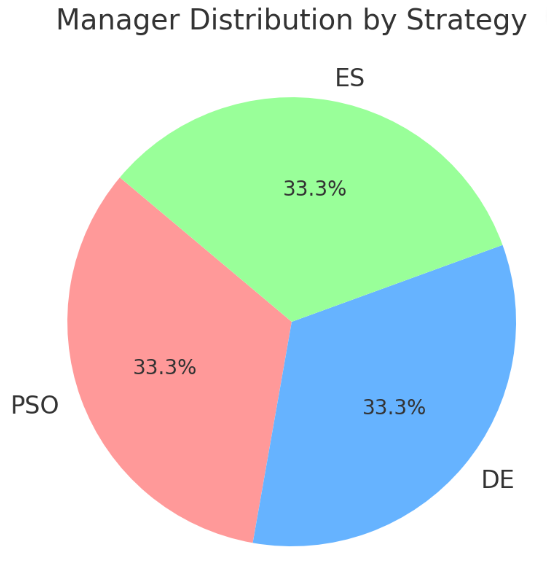
\includegraphics[width=0.6\linewidth]{plot/manager_distribution.png}
			\caption{Distribution of Managers by Strategy.}
		\end{figure}
	\end{frame}
	
	%%%%%%%%%%%%%%%%%%%%%%%%%%%%%%%%%%%%%%%%%%%%%%%
	\begin{frame}{Graphical Analysis: Player Score Distribution}
		\begin{figure}[H]
			\centering
			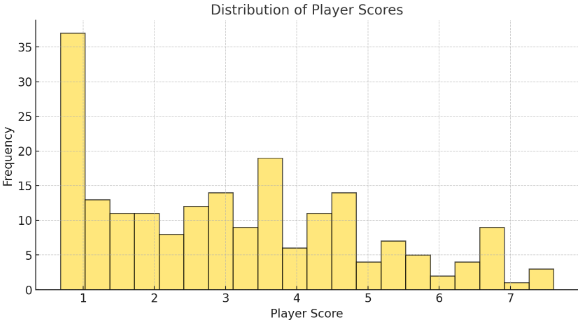
\includegraphics[width=0.8\linewidth]{plot/player_score_distribution.png}
			\caption{Distribution of Player Scores.}
		\end{figure}
	\end{frame}
	
	%%%%%%%%%%%%%%%%%%%%%%%%%%%%%%%%%%%%%%%%%%%%%%%
	\begin{frame}{Graphical Analysis: Budget Usage}
		\begin{figure}[H]
			\centering
			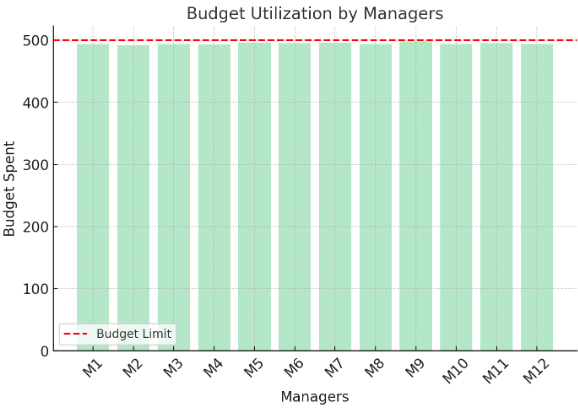
\includegraphics[width=0.8\linewidth]{plot/budget_usage.png}
			\caption{Budget Usage by Managers.}
		\end{figure}
	\end{frame}
	
	%%%%%%%%%%%%%%%%%%%%%%%%%%%%%%%%%%%%%%%%%%%%%%%
	\begin{frame}{Graphical Analysis: Forced Assignments}
		\begin{figure}[H]
			\centering
			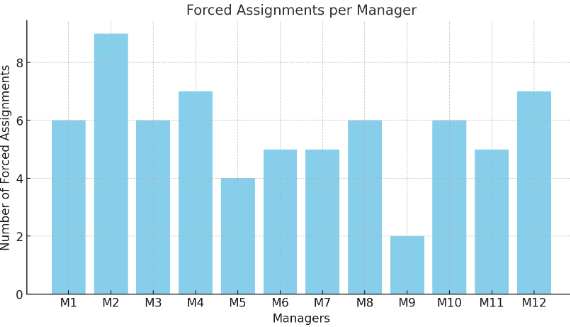
\includegraphics[width=0.8\linewidth]{plot/forced_assignments.png}
			\caption{Number of Forced Assignments per Manager.}
		\end{figure}
	\end{frame}
	
	%%%%%%%%%%%%%%%%%%%%%%%%%%%%%%%%%%%%%%%%%%%%%%%
	\begin{frame}{Graphical Analysis: Average Team Score}
		\begin{figure}[H]
			\centering
			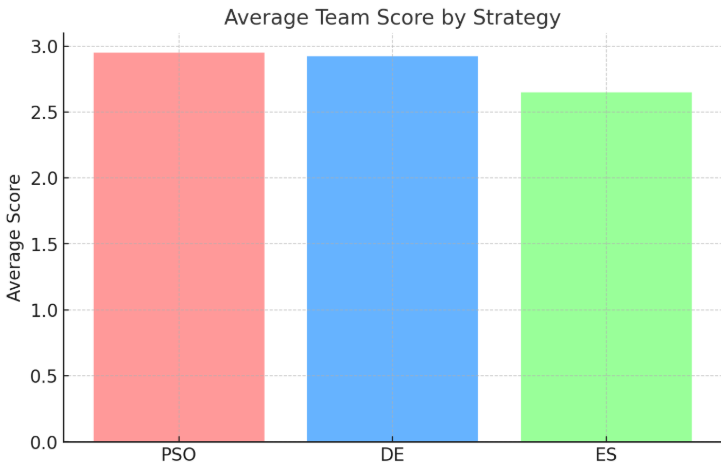
\includegraphics[width=0.8\linewidth]{plot/average_team_score_strategy.png}
			\caption{Average Team Score by Strategy (PSO, DE, ES).}
		\end{figure}
	\end{frame}
	
	%%%%%%%%%%%%%%%%%%%%%%%%%%%%%%%%%%%%%%%%%%%%%%%
	\begin{frame}{Tabular Analysis: Manager Recap}
		\begin{table}[H]
			\centering
			\caption{Manager Recap Table}
			\begin{tabular}{lrrrrr}
				\toprule
				\textbf{Manager} & \textbf{Strat} & \textbf{Forced} & \textbf{Spent} & \textbf{Leftover} & \textbf{Objective} \\
				\midrule
				Manager\_1  & PSO & 6 & 494.0 & 0.0 & 52.91 \\
				Manager\_2  & DE  & 9 & 492.0 & 0.0 & 51.48 \\
				Manager\_3  & PSO & 6 & 494.0 & 0.0 & 44.46 \\
				Manager\_4  & DE  & 7 & 493.0 & 0.0 & 53.64 \\
				Manager\_5  & ES  & 4 & 496.0 & 0.0 & 49.18 \\
				Manager\_6  & ES  & 5 & 495.0 & 0.0 & 46.02 \\
				Manager\_7  & PSO & 5 & 496.0 & 0.0 & 47.00 \\
				Manager\_8  & DE  & 6 & 494.0 & 0.0 & 55.32 \\
				Manager\_9  & ES  & 2 & 498.0 & 0.0 & 44.23 \\
				Manager\_10 & DE  & 6 & 494.0 & 0.0 & 46.59 \\
				Manager\_11 & ES  & 5 & 495.0 & 0.0 & 39.99 \\
				Manager\_12 & PSO & 7 & 494.0 & 0.0 & 53.23 \\
				\bottomrule
			\end{tabular}
		\end{table}
	\end{frame}
	
	%%%%%%%%%%%%%%%%%%%%%%%%%%%%%%%%%%%%%%%%%%%%%%%
	\begin{frame}{Tabular Analysis: Performance by Strategy}
		\begin{table}[H]
			\centering
			\caption{Performance by Strategy}
			\begin{tabular}{lrrr}
				\toprule
				\textbf{Strategy} & \textbf{Managers} & \textbf{Avg Total Score} & \textbf{Avg Team Score} \\
				\midrule
				PSO & 4 & 49.40 & 2.95 \\
				DE  & 4 & 51.76 & 2.92 \\
				ES  & 4 & 44.85 & 2.65 \\
				\bottomrule
			\end{tabular}
		\end{table}
	\end{frame}
	
	%%%%%%%%%%%%%%%%%%%%%%%%%%%%%%%%%%%%%%%%%%%%%%%
	\begin{frame}{Tabular Analysis: Player Score Summary}
		\begin{table}[H]
			\centering
			\caption{Player Score Summary}
			\begin{tabular}{lccc}
				\toprule
				& \textbf{Best} & \textbf{Worst} & \textbf{Average} \\
				\midrule
				Player Scores & 12.90 & 0.68 & 2.80 \\
				\bottomrule
			\end{tabular}
		\end{table}
	\end{frame}
	
	%%%%%%%%%%%%%%%%%%%%%%%%%%%%%%%%%%%%%%%%%%%%%%%
	\begin{frame}{Overall Discussion}
		\begin{itemize}
			\item \textbf{Manager Distribution:} A balanced manager distribution ensures diverse search behavior.
			\item \textbf{Player Score Distribution:} Highlights the need for careful budget allocation.
			\item \textbf{Budget Usage and Forced Assignments:} Indicate effective resource management.
			\item \textbf{Average Team Score:} All strategies (PSO, DE, ES) perform competitively.
			\item \textbf{Player Score Summary:} Only a few players achieve elite performance, emphasizing strategic selection.
		\end{itemize}
	\end{frame}
	
	%%%%%%%%%%%%%%%%%%%%%%%%%%%%%%%%%%%%%%%%%%%%%%%
	\begin{frame}{Conclusions and Future Directions}
		\begin{block}{Conclusions}
			\begin{itemize}
				\item Effective integration of metaheuristics with inverse optimization.
				\item Balanced approach towards budget, position constraints, and overall score.
			\end{itemize}
		\end{block}
		\begin{block}{Future Work}
			\begin{itemize}
				\item Develop a user-friendly GUI or web interface.
				\item Provide suggestions for optimal starting lineups.
				\item Explore hybrid approaches and reinforcement learning techniques.
			\end{itemize}
		\end{block}
	\end{frame}
	
	%%%%%%%%%%%%%%%%%%%%%%%%%%%%%%%%%%%%%%%%%%%%%%%
	\begin{frame}{Questions?}
		\centering
		\Large Thank you for your attention!
	\end{frame}
	
\end{document}
